20. Да, можно. Представим, что две вершины внутреннего треугольника и левая вершина внешнего треугольника лежат на окружности радиусом 566 с центром в нижней вершине.
\begin{figure}[ht!]
\center{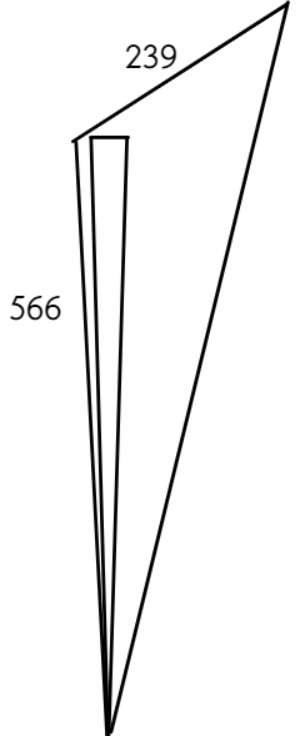
\includegraphics[scale=0.35]{g20.png}}
\end{figure}\newpage\noindent
